\documentclass{standalone}
\usepackage{tikz}
\usepackage{amsmath}

\begin{document}
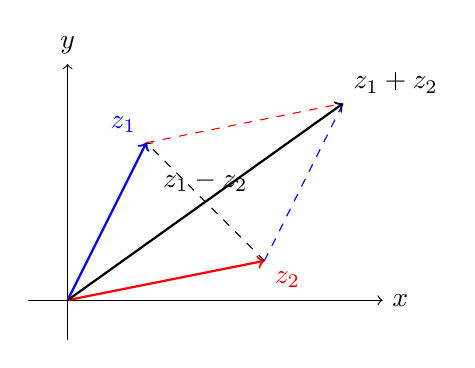
\begin{tikzpicture}[scale=1] % Adjust scale as needed

  % Axes
  \draw[->] (-0.5,0) -- (4,0) node[right] {$x$};
  \draw[->] (0,-0.5) -- (0,3) node[above] {$y$};

  % Vector z1 (blue)
  \draw[->, blue, thick] (0,0) -- (1,2) node[above left] {$z_1$};

  % Vector z2 (red)
  \draw[->, red, thick] (0,0) -- (2.5,0.5) node[below right] {$z_2$};

  % Vector z1 + z2 (black)
  \draw[->, black, thick] (0,0) -- (3.5,2.5) node[above right] {$z_1 + z_2$};

  % Vector z1 - z2 (black, dashed)
  \draw[->, black, dashed] (2.5,0.5) -- (1,2) node[midway, above] {$z_1 - z_2$};

  % Parallelogram (dashed, red and blue lines)
  \draw[dashed, red] (1,2) -- (3.5,2.5);
  \draw[dashed, blue] (2.5,0.5) -- (3.5,2.5);

\end{tikzpicture}
\end{document}